\documentclass{article}
\usepackage{amsmath}
\usepackage[utf8]{inputenc}
\usepackage{graphicx} % Comandos para manejar imágenes
\graphicspath{ {./images/} } % Carpeta de imágenes
\usepackage[table,xcdraw]{xcolor}
\setlength{\parskip}{2mm} % Espaciado

\usepackage[utf8]{inputenc}
\usepackage{geometry}
    \geometry{left=3cm,right=2cm,top=2cm,bottom=2cm}
%
\usepackage[spanish]{babel}
%
\usepackage[fixlanguage]{babelbib}
    \bibliographystyle{babunsrt}
%

\usepackage{floatrow}
\floatsetup[table]{style=plaintop}

\usepackage{url}

\usepackage[top=2cm, bottom=2.5cm, right=3 cm, left=3 cm]{geometry} % margenes

\usepackage{parskip} % Sangria

\title{Seminario siete: Optimizando Redes de Transporte, metro para Concepción, ciclovías para Valparaíso: comentarios sobre la presentación del Doctor Gabriel Gutierrez}
\author{Cristóbal Galleguillos Ketterer$^{1}$\\
\small{$^{1}$Industrial PhD Program}\\
\small{Pontificia Universidad Católica de Valparaíso}\\
\small{cristobal.galleguillos@pucv.cl}
}
\date{\small{\today}}

\begin{document}

\maketitle

\section{Introducción}

Como pocos casos, el transporte público, es una de las políticas sociales más ambiciosas en cuanto a costos y que más aportan a la igualdad social.Esto se manifiesta particularmente en ciudades extensas, donde los servicios se encuentran en las zonas centrales y los lugares donde las personas pernoctan en las afueras de los grandes centros urbanos.

El trabajo del doctor Gutiérrez presenta, el desarrollo de modelos de optimización, para determinar alternativas de transporte público optimizadas, para las ciudades de Concepción y Valparaíso. Considerando vías rápidas, líneas de metro, funiculares y ciclovías.

\section{Revisión de la literatura}

A partir del trabajo presentamos el grafo tipo árbol que permite ver las relaciones de la publicación con sus referencias y citas (Figura \ref{arb}).

\begin{figure}[H]
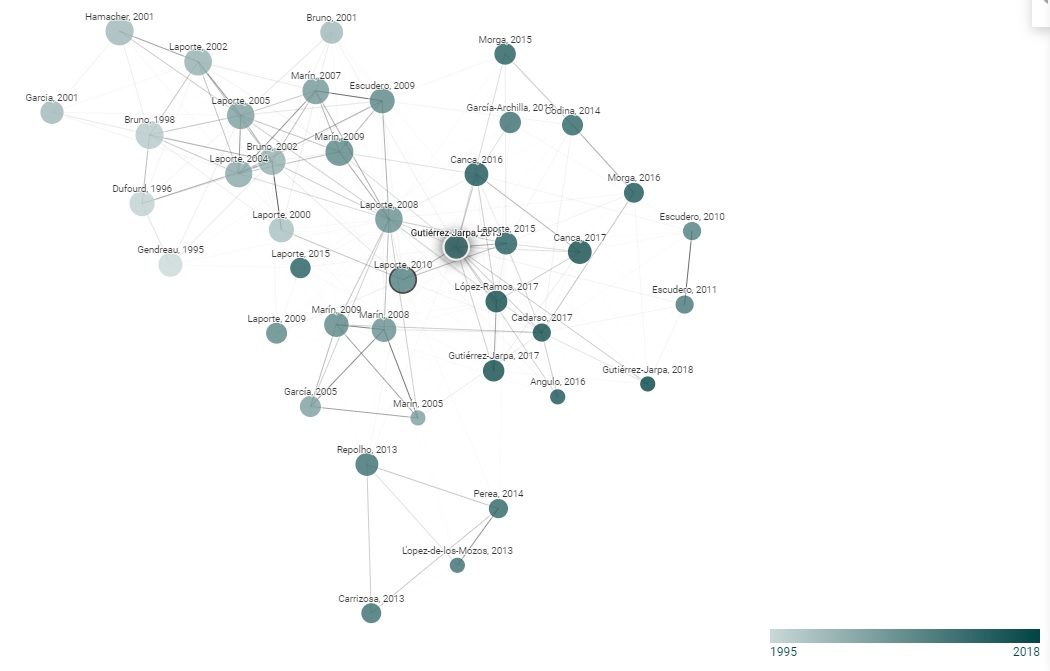
\includegraphics[scale=0.45]{Images/Arbol Gabriel.jpg}
\centering
\caption{Arbol de referencias y citas de \cite{article1}}
\label{arb}
\end{figure}

Considerando esto, resaltamos cuales son las fuentes más importantes, hacemos notar que la primera de ellas es un libro de texto clásico (Figura \ref{mas}).

\begin{figure}[H]
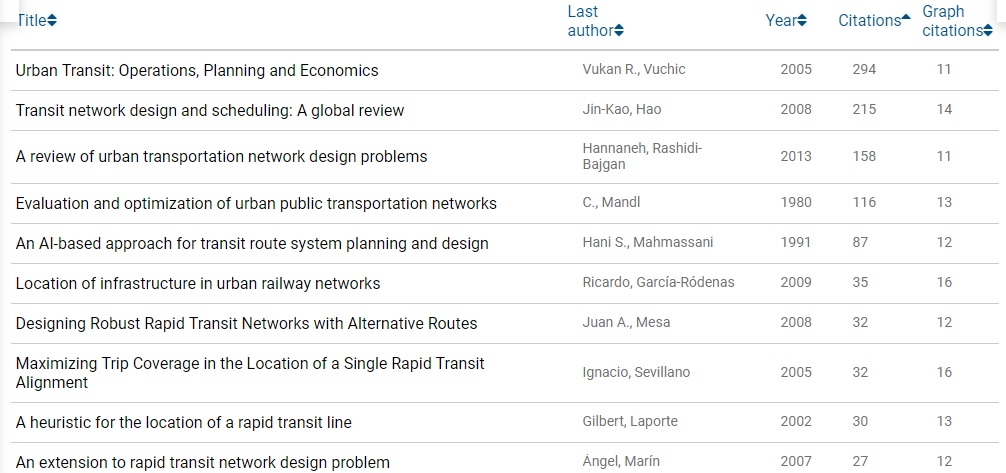
\includegraphics[scale=0.5]{Images/Citas.jpg}
\centering
\caption{Árticlos mas citados en árbol de \cite{article1}}
\label{mas}
\end{figure}

Finalmente se ha decidido presentar dentro del análisis bibliográfico, una revisión de las publicaciones del ámbito 
\textsl{Management Science and Operations Research}, por \textsl{ Scimago}, esta organización desarrolla estadísticas que miden la importancia de las publicaciones científicas.
Sus principales indicadores son:
\begin{itemize}
\item SJR (SCImago Journal Rank): Este indicador expresa el promedio de citas ponderadas recibidas en el año seleccionado (en este caso 2019) por los documentos publicados en la revista seleccionada en los tres años anteriores
\item Índice H: Este valor expresa el número de artículos (h) de la revista que han recibido al menos h citas. Cuantifica tanto la productividad científica de la revista como el impacto. Se presenta la figura de citada por Scimago [4].
\end{itemize}

\begin{figure}[H]
\includegraphics[scale=0.5]{Images/300px-H-index-es.svg.png}
\centering
\caption{Índice H, Fuente [4]}
\label{mas}
\end{figure}

Además se indican los cuartiles en que se ubican las revistas de acuerdo a los índices de impacto de acuerdo a una distribución de Poisson (ver Tabla \ref{table:indice}).

% Please add the following required packages to your document preamble:
% \usepackage{booktabs}
\begin{table}[H]
\caption{Ranking Scimago revistas categoría \textsl{Management Science and Operations Research} }
\begin{tabular}{@{}lllll@{}}
\hline\hline %inserts double horizontal lines
\toprule
\multicolumn{1}{c}{Ranking} & \multicolumn{1}{c}{Título} & \multicolumn{1}{c}{SJR} & \multicolumn{1}{c}{Cuartil} & \multicolumn{1}{c}{Índice H} \\ \midrule
\multicolumn{1}{|l|}{1} & \multicolumn{1}{l|}{Manufacturing and Service Operations Management} & \multicolumn{1}{l|}{5,732} & \multicolumn{1}{l|}{Q1} & \multicolumn{1}{l|}{77} \\ \midrule
\multicolumn{1}{|l|}{2} & \multicolumn{1}{l|}{Management Science} & \multicolumn{1}{l|}{5,439} & \multicolumn{1}{l|}{Q1} & \multicolumn{1}{l|}{237} \\ \midrule
\multicolumn{1}{|l|}{3} & \multicolumn{1}{l|}{Journal of Operations Management} & \multicolumn{1}{l|}{3,957} & \multicolumn{1}{l|}{Q1} & \multicolumn{1}{l|}{181} \\ \midrule
\multicolumn{1}{|l|}{4} & \multicolumn{1}{l|}{Surveys in Operations Research and Management Science} & \multicolumn{1}{l|}{3,583} & \multicolumn{1}{l|}{Q1} & \multicolumn{1}{l|}{21} \\ \midrule
\multicolumn{1}{|l|}{5} & \multicolumn{1}{l|}{Operations Research} & \multicolumn{1}{l|}{3,539} & \multicolumn{1}{l|}{Q1} & \multicolumn{1}{l|}{128} \\ \midrule
\multicolumn{1}{|l|}{6} & \multicolumn{1}{l|}{Transportation Research, Part C: Emerging Technologies} & \multicolumn{1}{l|}{3,342} & \multicolumn{1}{l|}{Q1} & \multicolumn{1}{l|}{116} \\ \midrule
\multicolumn{1}{|l|}{7} & \multicolumn{1}{l|}{Research Policy} & \multicolumn{1}{l|}{3,246} & \multicolumn{1}{l|}{Q1} & \multicolumn{1}{l|}{224} \\ \midrule
\multicolumn{1}{|l|}{8} & \multicolumn{1}{l|}{Transportation Research Part B: Methodological} & \multicolumn{1}{l|}{2,895} & \multicolumn{1}{l|}{Q1} & \multicolumn{1}{l|}{130} \\ \midrule
\multicolumn{1}{|l|}{9} & \multicolumn{1}{l|}{Journal of Management Information Systems} & \multicolumn{1}{l|}{2,863} & \multicolumn{1}{l|}{Q1} & \multicolumn{1}{l|}{137} \\ \midrule
\multicolumn{1}{|l|}{10} & \multicolumn{1}{l|}{Production and Operations Management} & \multicolumn{1}{l|}{2,843} & \multicolumn{1}{l|}{Q1} & \multicolumn{1}{l|}{102} \\ \midrule
\multicolumn{1}{|l|}{11} & \multicolumn{1}{l|}{Omega} & \multicolumn{1}{l|}{2,579} & \multicolumn{1}{l|}{Q1} & \multicolumn{1}{l|}{131} \\ \midrule
\multicolumn{1}{|l|}{12} & \multicolumn{1}{l|}{International Journal of Production Economics} & \multicolumn{1}{l|}{2,379} & \multicolumn{1}{l|}{Q1} & \multicolumn{1}{l|}{172} \\ \midrule
\multicolumn{1}{|l|}{13} & \multicolumn{1}{l|}{European Journal of Operational Research} & \multicolumn{1}{l|}{2,364} & \multicolumn{1}{l|}{Q1} & \multicolumn{1}{l|}{243} \\ \midrule
\multicolumn{1}{|l|}{14} & \multicolumn{1}{l|}{Journal of Business Logistics} & \multicolumn{1}{l|}{2,344} & \multicolumn{1}{l|}{Q1} & \multicolumn{1}{l|}{65} \\ \midrule
\multicolumn{1}{|l|}{15} & \multicolumn{1}{l|}{Transportation Research Part E: Logistics and Transportation Review} & \multicolumn{1}{l|}{2,302} & \multicolumn{1}{l|}{Q1} & \multicolumn{1}{l|}{103} \\ \midrule
\multicolumn{1}{|l|}{16} & \multicolumn{1}{l|}{Transportation Research Part A: Policy and Practice} & \multicolumn{1}{l|}{2,109} & \multicolumn{1}{l|}{Q1} & \multicolumn{1}{l|}{120} \\ \midrule
\multicolumn{1}{|l|}{17} & \multicolumn{1}{l|}{EURO Journal on Transportation and Logistics} & \multicolumn{1}{l|}{2,1} & \multicolumn{1}{l|}{Q1} & \multicolumn{1}{l|}{16} \\ \midrule
\multicolumn{1}{|l|}{18} & \multicolumn{1}{l|}{Journal of Informetrics} & \multicolumn{1}{l|}{2,079} & \multicolumn{1}{l|}{Q1} & \multicolumn{1}{l|}{65} \\ \midrule
\multicolumn{1}{|l|}{19} & \multicolumn{1}{l|}{International Journal of Production Research} & \multicolumn{1}{l|}{1,776} & \multicolumn{1}{l|}{Q1} & \multicolumn{1}{l|}{125} \\ \midrule
\multicolumn{1}{|l|}{20} & \multicolumn{1}{l|}{Mathematics of Operations Research} & \multicolumn{1}{l|}{1,727} & \multicolumn{1}{l|}{Q1} & \multicolumn{1}{l|}{73} \\ \midrule
\multicolumn{1}{|l|}{21} & \multicolumn{1}{l|}{Computers and Operations Research} & \multicolumn{1}{l|}{1,663} & \multicolumn{1}{l|}{Q1} & \multicolumn{1}{l|}{143} \\ \midrule
\multicolumn{1}{|l|}{22} & \multicolumn{1}{l|}{Proceedings of the Annual ACM-SIAM Symposium on Discrete Algorithms} & \multicolumn{1}{l|}{1,517} & \multicolumn{1}{l|}{-} & \multicolumn{1}{l|}{15} \\ \midrule
\multicolumn{1}{|l|}{23} & \multicolumn{1}{l|}{Journal of Leadership and Organizational Studies} & \multicolumn{1}{l|}{1,504} & \multicolumn{1}{l|}{Q1} & \multicolumn{1}{l|}{39} \\ \midrule
\multicolumn{1}{|l|}{24} & \multicolumn{1}{l|}{INFORMS Journal on Computing} & \multicolumn{1}{l|}{1,476} & \multicolumn{1}{l|}{Q1} & \multicolumn{1}{l|}{75} \\ \midrule
\multicolumn{1}{|l|}{25} & \multicolumn{1}{l|}{Quality Technology and Quantitative Management} & \multicolumn{1}{l|}{1,421} & \multicolumn{1}{l|}{Q1} & \multicolumn{1}{l|}{16} \\ \midrule
\hline %inserts single line
\end{tabular}
\label{table:indice}
\end{table}

La publicación \cite{article1}, está editada por una revista de alto impacto ubicada en la posición 25 según la Tabla \ref{table:indice}

\section{Marco teórico}

La programación lineal entera mixta (MILP, por sus siglas en inglés) es una herramienta muy utilizada para resolver problemas de maximización (o minimización) donde el conjunto de soluciones factibles es discreto. 
En este caso las funciones objetivo son lineales y las restricciones que definen el problema también, por otro lado las variables de decisión, pueden continuas o discretas. Una formulación estándar se presenta a continuación \cite{article3} .

\begin{equation}
min=c^{T}x+d^{T}y 
\label{min}
\end{equation}

S.t.

\begin{equation*}
\textbf{Ax+Ey}=
\begin{bmatrix}
\leq \\
= \\
\geq 
\end{bmatrix}
\textbf{b}
\end{equation*}

\begin{equation}
x_{min}\leq x \leq x_{max} \;\;\;\; \textbf{y}\in \{0,1\}^{n_{y}} 
\end{equation}

Estos problemas presentan una alta dificultad de resolución, y a menudo grandes capacidades de cómputo. Entre los ejemplos de modelos que utilizan este tipo de programación lineal encontramos 
Planificación de la producción.
Distribución de energía eléctrica.
Distribución de combustible.
Redes de transporte.
El trabajo presentado por el doctor Gutiérrez, consiste en el diseño de redes de transporte rápido (RTNDP), la contribuciones del profesor serán presentadas en el siguiente apartado.


\section{Contribución del autor}

La investigación del profesor Gutiérrez, se desarrolla en el marco de la optimización de sistemas de transporte de macro ciudades de Chile, en este caso particular, Concepción y Valparaíso, ambas ciudades tienen características similares: Son el centro de metrópolis conurbadas, carecen de redes formales de metro (Biotrén en Concepción, Figura \ref{Bio} y Merval, Figura \ref{mer} en Valparaíso, tienen mayormente características de servicios de trenes de cercanías).

\begin{figure}[H]
\includegraphics[scale=1]{Images/Mapa_Biotren.png}
\centering
\caption{Red Biotren, Fuente Biotren}
\label{Bio}
\end{figure}

\begin{figure}[H]
\includegraphics[scale=0.5]{Images/512px-MetroValparaíso.svg.png}
\centering
\caption{Red Merval, Fuente Merval}
\label{mer}
\end{figure}

Los modelos propuestos pretenden buscan la ubicación óptima de estaciones, de modo que la red resultante considere la optimización de: minimizar los costos de construcción, maximizar la demanda capturada considerando los flujos de origen y destino y maximizar el tiempo ahorrado por la demanda capturada.

Las restricciones aseguran la estructura de la red, las asignaciones, el tiempo y la captura de tráfico.

De este trabajo original se desprenden dos interesantes extensiones.

En la primera, se asocia de forma directa a una red de metro, donde 
el modelo de optimización se basa en cuatro pasos, el primero generar de modo optimista el mayor número de redes para las condiciones determinadas, en segundo lugar se realizan las estimaciones de viaje origen destino, y la demanda capturada. A partir de estos datos se seleccionad los corredores ajustados a la demanda real y finalmente se definen las estaciones de trasferencia.

Los trabajos previos fueron desarrollados para la ciudad de Concepción, se presenta una figura con la red optimizada del trabajo (Figura \ref{conce}), se puede comprar con (Figura \ref{mer}).

\begin{figure}[H]
\includegraphics[scale=0.5]{Images/estrellaCOnce.jpg}
\centering
\caption{Resultado modelación para Concepción, Fuente \cite{article1}}
\label{conce}
\end{figure}

La segunda extensión, consiste en ampliar el pool de medios de transporte incorporando ciclovías y funiculares, esta continuación del trabajo deviene de las características geográficas naturales de Valparaíso. El modelo minimiza los costos de construcción de las estaciones de funicular, el costo de las ciclovías y el costo de las estaciones para bicicletas y maximiza el flujo por los nuevos corredores.

El resultado se puede apreciar en la Figura \ref{valpo} (en rojo las ciclovias y en verde los funiculares, nótese que la red de ciclovias recorre el denominado "Plan" de Valparaíso)

\begin{figure}[H]
\includegraphics[angle=180, scale=0.5]{Images/final valpo.jpg}
\centering
\caption{Resultado modelación para Valparaíso, Fuente \cite{article2}}
\label{valpo}
\end{figure}

\section{Comentarios}

Las potenciales extensiones a este trabajo fueron ampliamente comentadas en durante la conferencia, una de ellas es como se incorporan a la estructura del modelo aspectos relativos al financiamiento, tales como la estructura de precios sociales (ex- Metodología MIDEPLAN), o el mecanismo de concesiones públicas, o los modelos de inversión con recursos propios como los que tiene Metro de Santiago.

Otro aspecto interesante a considerar son los potenciales criterios de ubicación de estaciones que involucran incentivos no asociados a las optimización de los flujos de transporte ni los costos, como la cercanía a potenciales desarrollos urbanos, o bien especulaciones inmobiliarias.

En el caso de Metro de Santiago, en los últimos años se verifica que Metro diversifica su funciones como un agente inmobiliario mas, obteniendo recaudaciones por arriendo de locales comerciales u otros, estos servicios adicionales se podrían incluir en las modelaciones como ingresos asociados a el marco urbano en que se encuentran las potenciales estaciones.




\nocite{*}
    \bibliography{src/ref}

\end{document}
